% Source: tex/chapters/ch05/09_開発プロセスと適用領域におけるテスト.tex
\subsubsection{ソフトウェア開発プロセス内のテスト}
\paragraph{従来型プロセスにおけるテスト}
逐次型、V 字型、スパイラル、反復型などの従来型プロセスでは、テストが一つの活動として明確に位置づけられることが多い。後半で集中的にテストする場合、利用者ニーズとのずれや評価上の問題が遅く見つかるリスクがある。品質を評価し制御するために、TMMi、SPI、SPICE、CMMI、統一プロセスなどの成熟度モデルや改善枠組みが用いられてきた。

\paragraph{シフトレフトに沿ったテスト}
シフトレフトは、開発の早い段階でテストを採用し、欠陥を早く検出して除去する考え方である。アジャイル、DevOps、TDD はこの動きに含まれる。内部コード品質では、単体・結合テストや構造ベース技法が重要である。業務ニーズでは、システム・受入テスト、利用ベース技法、シナリオベース技法が重要である。知覚品質では、アルファ、ベータ、導入、使いやすさ、セキュリティ、プライバシーが重視される。品質保証では、性能、セキュリティ、プライバシー、適合性、順守が対象になる。

アジャイル開発では、顧客やチームメンバーを含む関係者がテスト活動に関与し、回帰欠陥のリスクや変化する要求への対応が重要になる。TDD では、コードを書く前にテストケースを作り、要求の理解を明確化する。DevOps や継続的インテグレーションでは、回帰テストやスモークテストを継続的に行い、配備前に基本的なテスト可能性を確認する。

\begin{figure}[htbp]
\centering
\IfFileExists{assets/generated_figures/ch05/fig-ch05-13.png}{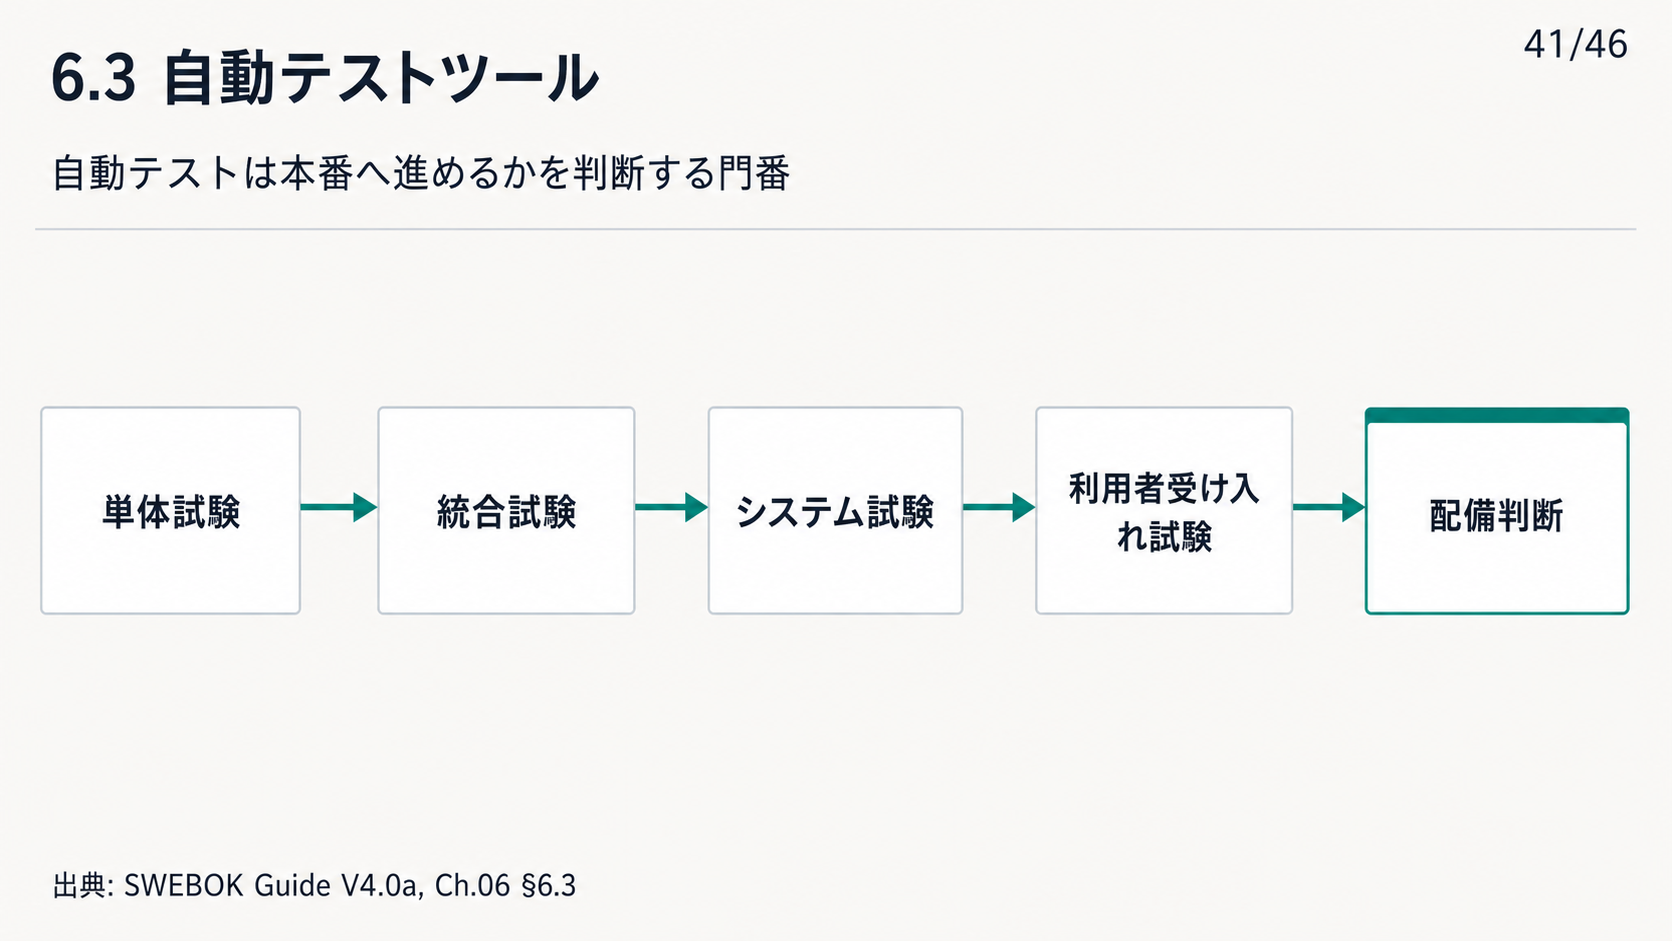
\includegraphics[width=0.96\linewidth]{assets/generated_figures/ch05/fig-ch05-13.png}}{\fbox{\parbox[c][48mm][c]{0.9\linewidth}{\centering 画像生成待ち\\従来型とシフトレフトの比較図}}}
\caption{従来型とシフトレフトの比較図}
\label{fig:ch05-13}
\end{figure}
